%&pdflatex
\documentclass[preprint,3p,review,authoryear,10pt]{elsarticle}

\usepackage{graphicx}
\usepackage{natbib}
\usepackage{setspace}
\usepackage{multirow}
\usepackage{booktabs}
\usepackage[T1]{fontenc}
%\setlength{\parindent}{0in}
\usepackage{times}
\usepackage[british]{babel}
\usepackage{algorithm}
\usepackage{algorithmic} \renewcommand{\algorithmicrequire}{\textbf{Given:}} \renewcommand{\algorithmicensure}{\textbf{Returns:}}
\usepackage{amsfonts}
\usepackage{mathrsfs}
\usepackage{amssymb}
\usepackage{amsmath}
\usepackage{mathtools}
\renewcommand \thesection{\arabic{section}}
\usepackage[caption=false]{subfig}
\usepackage[compact]{titlesec}
\usepackage{soul}
\usepackage{textcomp}
\usepackage[section]{placeins}
\usepackage{url}
\usepackage{xspace}
\usepackage{lineno}
\usepackage{hyperref}
    \hypersetup{colorlinks=true,linkcolor=green}
\usepackage{cleveref}

%Added by Diarmid
\usepackage{siunitx}


% % new commands
\newcommand{\I}{\mathcal{I}}
\DeclareMathOperator*{\any}{any}
\DeclareMathOperator*{\all}{all}

\newcommand{\ddt}[1]{\frac{\partial #1}{\partial t}}
\newcommand{\ddx}[1]{\frac{\partial #1}{\partial x}}

%% for annotating paper for TODO notes etc.  Comment this out and
%% uncomment alternative for final version
\newcommand{\sol}[1]{\footnote{#1}\marginpar{\fbox{\thefootnote}}}


\journal{Computers \& Chemical Engineering}

\begin{document}
\linenumbers


\title{MILP for idling to minimise coulombic losses}

\section{MILP formulation with fixed coulombic losses}
In the NLP formulation introduced in XX, it is assumed that the coulombic efficiency of the RFB is constant, i.e. the coulombic losses are proportional to the useful current density. \textit{What I say in assumptions section of paper...}

In order to address this concern, the SOC at time $t$ was redefined by:

\begin{equation}
\label{eqn: Method_MINLP_SOC_Tracker}
SOC_t = SOC_{t-1} +\frac{A.\tau}{1000C}(I_{C, t} - I_{D, t} - \delta_tl_C) \forall t \in Y
\end{equation}

Where $\delta_t$ is a binary indicator variable with 0 indicating an idle state and 1 an active state, and $l_C$ the fixed coulombic loss term (\si{\ampere}). It is assumed that the volume of electrolyte in the stack is negligible compared to the volume in the reservoirs.

The condition that the charging or discharging of the RFB requires the system to be in the active state is formalised by:

\begin{equation}
\begin{split}
    \label{eqn: On_off_condition}
    I_{C,t} > 0 \implies \delta_t = 1\\
    I_{D,t} > 0 \implies \delta_t = 1
    \end{split}
\end{equation}

The constraints that enforce these conditions are defined by:

\begin{equation}
\begin{split}
    \label{eqn: on_off_constraint}
    I_{C,t} - I_{Max}\delta_{C,t} \leq 0\\ 
    I_{D,t} - I_{Max}\delta_{D,t} \leq 0
    \end{split}
\end{equation}

 after \cite{Williams2013}.
 
 The expression of coulombic losses as a fixed term results in the restriction of operation in the low current-density range, where the coulombic losses would cancel out the voltaic loss reductions. \cref{fig:MINLP_on_EffC} shows a comparison of the optimal schedules obtained using the NLP formulation in XX and the MINLP formulation.
 
 \begin{figure}[!ht]
\centering
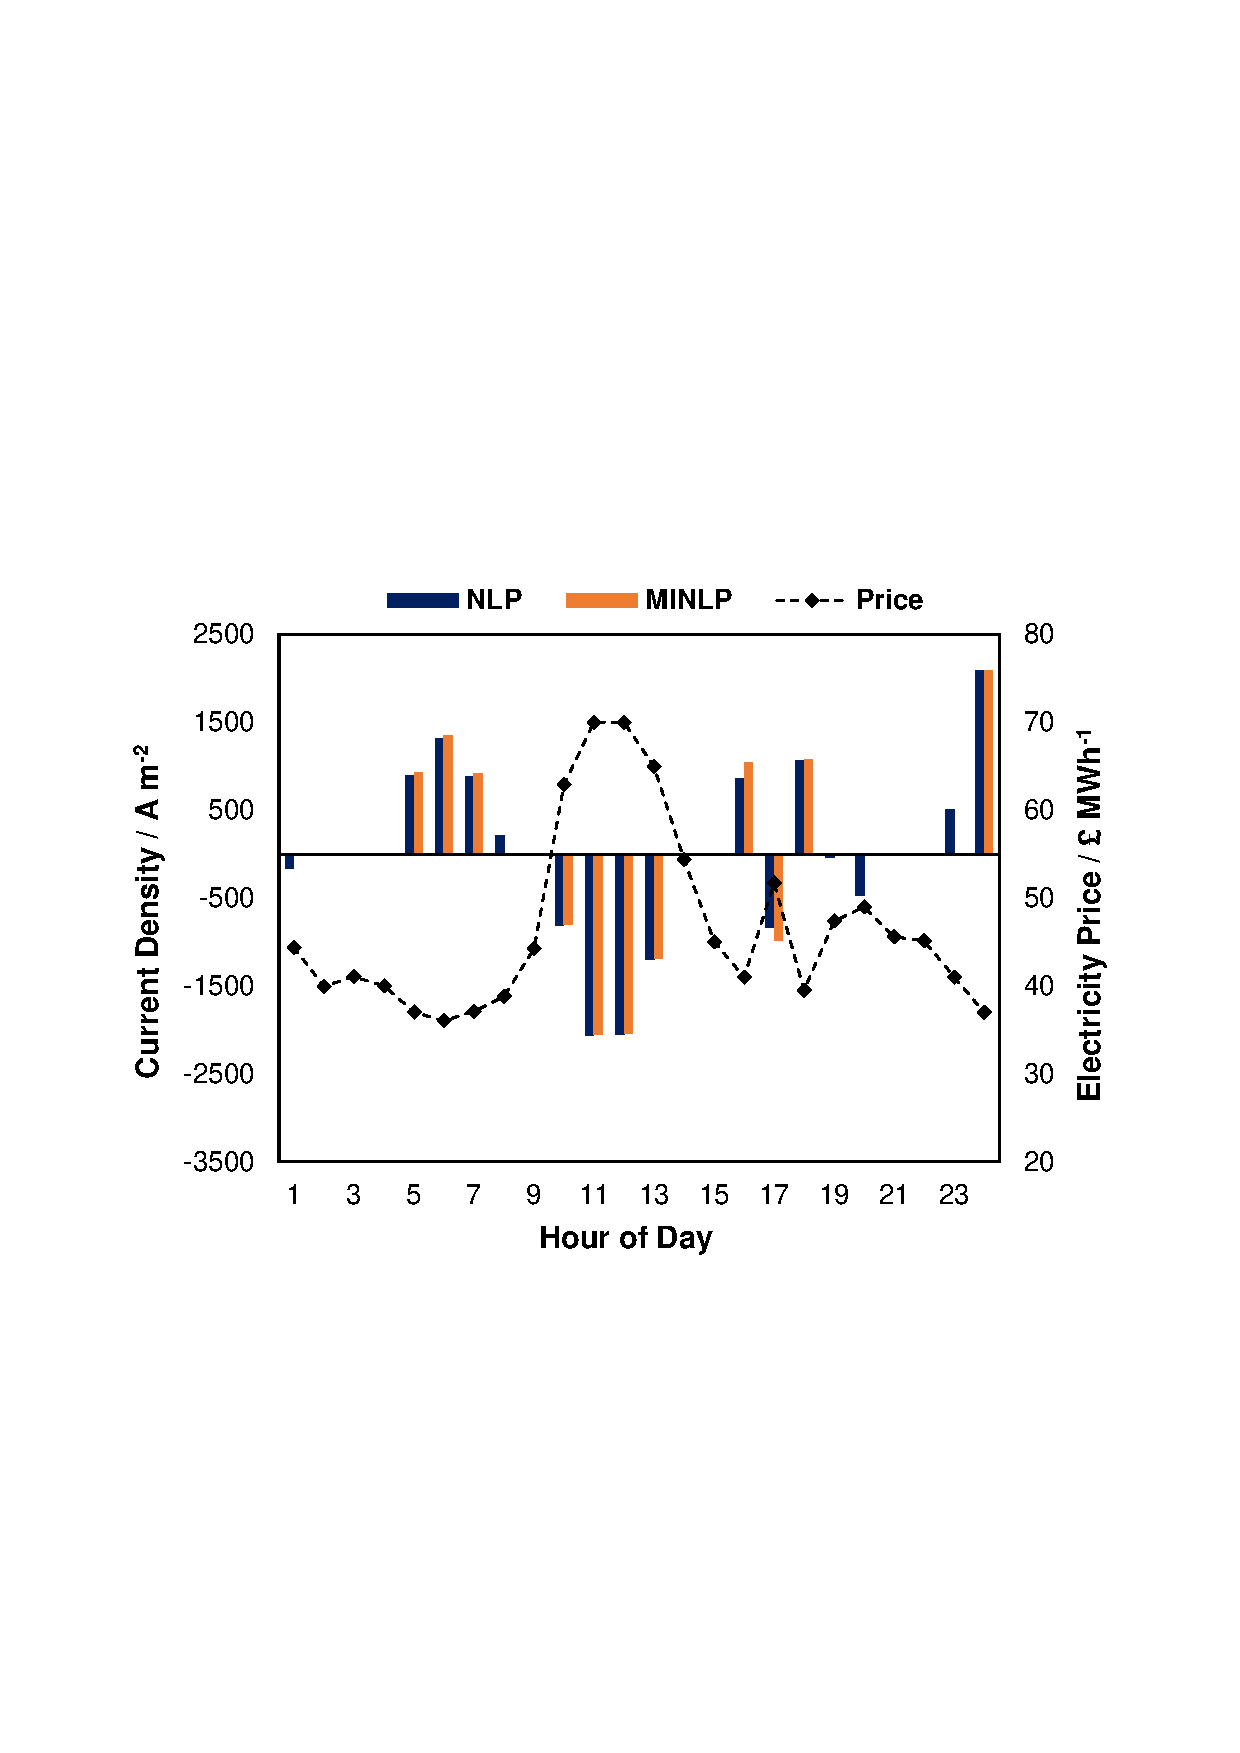
\includegraphics[trim = 2cm 8cm 2cm 9cm, clip, width = .5\textwidth]{./figures/MINLP_schedule.pdf}
\caption{Optimal schedules obtained by NLP and MINLP optimisation for N2EX electrical price on 22$^{nd}$ August 2017.}
\label{fig:MINLP_on_EffC}
\end{figure}
 
  
A similar approach may be employed to deal with other fixed losses, such as the pumping power loss for a constant output pump.
\end{document}
